% test-nouveautes.tex -- nouveautés de tkz-graph et tkz-berge (étape 2)
% \tkzSetUpGraph, flèches, rotation, \tkzHighlightPath, matrice
% d'adjacence, \tkzGraphFromMatrix, \grProbMatrix, \grHypercube, \grTree
% Compile avec pdfLaTeX et LuaLaTeX.
\documentclass{article}
\usepackage[margin=1.5cm]{geometry}
\usepackage{tkz-berge}
\usetikzlibrary{arrows.meta}
\pagestyle{empty}
\begin{document}
\section*{1. \texttt{\string\tkzSetUpGraph}, flèches, rotation}
\begin{tikzpicture}
  \tkzSetUpGraph[medium size=14pt, vertex line color=blue, light fill=blue!10,
                 edge width=1pt, edge color=blue!60!black]
  \Vertices[unit=1.5,rotation=90]{circle}{A,B,C,D,E}
  \Edges[->](A,B,C)\Edge[<->](C)(D)\Edge[<-](D)(E)\Edge(E)(A)
\end{tikzpicture}\quad
\begin{tikzpicture}
  \tkzSetUpGraph[directed, arrow tip={Stealth[length=6pt]}]
  \Vertices[unit=1.5,rotation=90,clockwise]{circle}{A,B,C,D,E}
  \Edges(A,B,C,D,E)\Edge[-](E)(A)
\end{tikzpicture}\quad
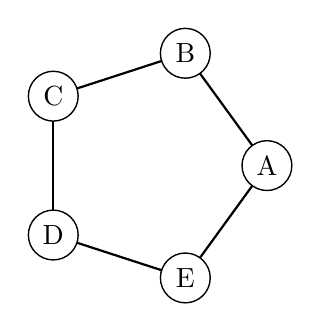
\begin{tikzpicture}             % les réglages précédents sont oubliés
  \Vertices[unit=1.5]{circle}{A,B,C,D,E}\Edges(A,B,C,D,E,A)
\end{tikzpicture}

\section*{2. \texttt{\string\tkzHighlightPath}}
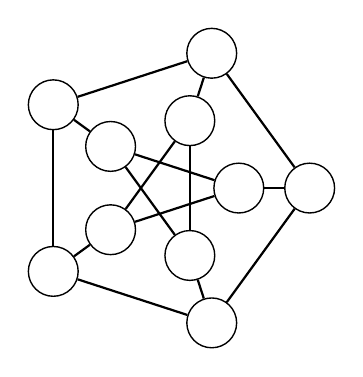
\begin{tikzpicture}[scale=.6]
  \GraphInit[vstyle=Normal]\SetVertexNoLabel
  \grPetersen[RA=3,RB=1.5]
  \tkzHighlightPath[cycle]{a0,a1,a2,a3,a4}
  \tkzHighlightPath[color=blue]{a0/b0,b2/b4}
\end{tikzpicture}\quad
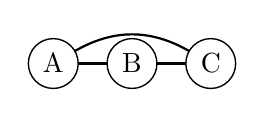
\begin{tikzpicture}
  \Vertices{line}{A,B,C}
  \Edge[style={bend left=30}](A)(C)\Edges(A,B,C)
  \tkzHighlightPath[color=orange,lw=2.5pt,style={bend left=30}]{A,C}
\end{tikzpicture}

\section*{3. Matrice d'adjacence}
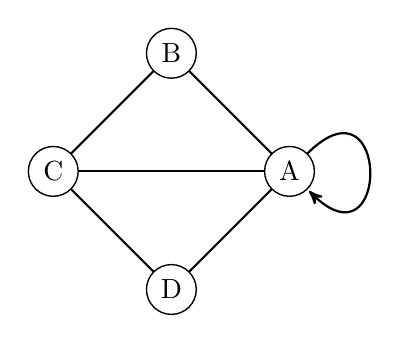
\begin{tikzpicture}
  \Vertices[unit=1.5]{circle}{A,B,C,D}
  \Edges(A,B,C,D,A)\Edge(A)(C)\Loop[dir=EA,dist=1.5cm](A)
\end{tikzpicture}
\quad $M = \tkzAdjacencyMatrix$ \quad
ordre imposé : \tkzAdjacencyMatrix[order={D,C,B,A}]

\medskip
\begin{tikzpicture}
  \tkzGraphFromMatrix[unit=1.5,rotation=90]{A,B,C,D}%
     {0,1,1,0;
      1,0,1,1;
      1,1,0,1;
      0,1,1,1}
\end{tikzpicture}\quad
\begin{tikzpicture}
  \tkzGraphFromMatrix[directed,weighted,unit=2]{1,2,3}%
     {0,4,0; 2,0,7; 5,0,0}
\end{tikzpicture}\quad
$\tkzAdjacencyMatrix[directed]$

\section*{4. Graphe probabiliste à 3 et 4 états}
\begin{tikzpicture}
  \grProbMatrix[unit=2,rotation=90]{A,B,C}%
     {0.5,0.3,0.2; 0.1,0.6,0.3; 0.4,0,0.6}
\end{tikzpicture}\qquad
\begin{tikzpicture}
  \SetVertexMath
  \grProbMatrix[unit=2.2,rotation=45,loop distance=1.2cm]{E_1,E_2,E_3,E_4}%
     {0.2,0.8,0,0; 0,0.5,0.5,0; 0,0,0.3,0.7; 1,0,0,0}
\end{tikzpicture}

\section*{5. Hypercubes}
\begin{tikzpicture}[scale=.8]
  \GraphInit[vstyle=Art]
  \grHypercube[RA=2]{1}
  \begin{scope}[xshift=3cm]\grHypercube[RA=2,prefix=b]{2}\end{scope}
  \begin{scope}[xshift=7cm]\grHypercube[RA=2.5,prefix=c]{3}\end{scope}
  \begin{scope}[xshift=12cm]\grHypercube[RA=2,prefix=d]{4}\end{scope}
\end{tikzpicture}

\begin{tikzpicture}
  \GraphInit[vstyle=Normal]\tkzSetUpGraph[medium size=20pt]
  \grHypercube[RA=3.5,prefix={}]{3}
  \tkzHighlightPath[cycle]{000,001,011,010,110,111,101,100}% code de Gray
\end{tikzpicture}\quad
\begin{tikzpicture}[scale=.7]
  \GraphInit[vstyle=Simple]\grHypercube[RA=2,rotation=22.5]{5}
\end{tikzpicture}

\section*{6. Arbres}
\begin{tikzpicture}[scale=.8]
  \GraphInit[vstyle=Normal]
  \grTree[RA=1.3,RB=1.5,Math]{2}{3}
\end{tikzpicture}\quad
\begin{tikzpicture}[scale=.8]
  \GraphInit[vstyle=Art]
  \grTree[RA=.7,RB=1.2,prefix=t]{3}{2}
  \tkzHighlightPath{t0;0,t1;2,t2;7}
\end{tikzpicture}
\end{document}
